





\section{Introduction}
\label{sec:introduction}


How do financial markets respond to war events?
How do the events within war, such as battles, lead to the termination of war?
This work addresses both of these questions in the context of the case of the American Civil War. 
The strategy of this work is to answer the first question in order to understand the second.
I estimate the effects of militarily significant battles on the yields of U.S. government bonds.
I argue that yields, and thus riskiness, of U.S. government bonds was almost certainly primarily driven by expecations of the cost of the war.
Thus, the bond yields of U.S. government can act as a proxy for expectations of the war cost given the available information at the time.
I estimate several models of incorporating the effects of battles on bond yields and find the following.
First, the effect of battles on bond yields, and by extension expectations of the war cost, was asymmetric.
On average, Confederate victories increased yields by approximately 5\%, while, on average, Union victories had little to no effect.
This is consistent with the asymmetric strategic environment of the American Civil War: the U.S. had to win battles to recapture the seceding states, while the Confederacy had to win to defend.
It also suggests that U.S. victories were expected by the market, while Confederate victories were surprising.
Second, the battles with the largest estimated effects on bond yields were those during the Overland and start of the Petersburg Campaign in May--June, 1864 in which Ulysses S. Grant's advance on the Confederate capital of Richmond was met with resistance.
Third, although including battles in the model improves the model fit both within-sample and prediction, the improvement is surprisingly small.
This is consistent with many events within a war, not just major battles, having an influence on war expectations.
I conclude with a suggestion of how natural language processing methods applied to newspapers may provide a better means of assessing the effects of war events, as observed by contemporaries, on war expectations.

The approach in this work, using financial markets to better understand war termination, is a general one that can used in the study of conflict.
Understanding theories of war initiation and termination requires an understanding of the means of war, military combat.
This is what \textcite{Gartner1998} calls ``opening up the black box of war.''
However, the empirical study of military combat within war has lagged behind the study of war initiation that treats war as a black box \parencite{Reiter2003}.
The approach taken in this work, using the prices of financial assets as a proxy for expectations of war termination, provides a method that helps deal with two problems in the study of military combat within war.
First, by providing a within-case time-varying measure of the expected war termination, it allows for the quantitative analysis of small numbers of cases.
This is useful because quality data on intra-war events is rare, making large-$n$ intra-war analysis difficult if not infeasible.
Due to the lack of multi-war intra-war data, the preferred approach to the empirical study of the bargaining theory of war with intra-war data has been qualitative case studies \parencites{Reiter2003}[][Chapter 9]{Reiter2009}. 
While there are some implications of the bargaining model of war that can be tested with within-case data, such as those regarding the offers made throughout the war, the use of within-case data prohibits the use of several key dependent variables of interest in these models---the cost, duration, and outcome of a war---since there is no variation in these variables within a single war.
Financial market data provides an alternative method with which to analyze the intra-war events using a single or small number of cases for which data is available.
Financial asset price data, when it can be shown to be a prediction of the war result, allows the researcher to estimate the effect of events on war outcomes by employing the prices of carefully chosen financial assets as a time-varying expectation of those war outcomes.
The second application is as a measure of surprising events.
Surprising events are particularly important in private information theories of war, but it is difficult to know what events were surprising to contemporaries \parencite{Shirkey2009a}.
Since prices of financial assets only respond to new information, they provide a natural measure of surprising events, which are particularly important in informational theories of war \parencite{Shirkey2009a}.

This work adds to an economic history literature on the effects of war events in the American Civil War on currencies and other financial assets \parencites{Mitchell1903}{Mitchell1908}{Schwab1901}{Roll1972}{Calomiris1988}{DavisPecquet1990}{WillardGuinnaneEtAl1996}{McCandless1996}{SmithSmith1997}{BrownBurdekin2000}{Weidenmier2000}{Weidenmier2002}{HaberMitchenerOosterlinckEtAl2014}.
This work contributes to that literature by using the yields of U.S. government bonds, which unlike Greenbacks, provide a time series that spans the entire war. 
This work estimates the effects of both Confederate and Union victories, as well as that of individual major battles.
Finally, it ties that literature to political science theories of war, and shows how those insights can be used not just to understand how markets work, but also to better understand how war works.
This work builds on a large and growing literature which measures impact or identifies important political events using financial \parencites{NorthWeingast1989}{north2000introd}{FreyKucher2000}{sussman2000instit}{wells2000revol}{Herron2000}{eldor2004finan}{ChenSiems2004}{Greenstone2007} or prediction markets \parencites{WolfersZitzewitz2004}{ArrowForsytheGorhamEtAl2008}{WolfersZitzewitz2009}.




\section{Financial Markets and the Study of War}
\label{sec:barg-theory-war}

Financial markets relate to the study of war in several ways.
First, they provide a measure of the the costs of war \parencites{SchneiderTroeger2006}{GuidolinLaFerrara2010}.
Second, financial markets are themselves a key actor or mechanism in several theories of war.
This includes the ``Capitalist Peace'' \parencites{Gartzke2007}{DafoeKelsey2014a}, in which markets can provides signals of the costs of war to actors, and \textcite{Slantchev2012a}, in which debt financing creates a commitment problem.
Third, in some cases, the prices of financial assets act similarly to a prediction market for the expected onset or outcome of war.
The implied expectations of war outcomes  derived from the prices of these financial assets can be used to assess theories of war initiation and termination.%
\footnote{See Chapter~\ref{cha:financ-mark-onset} for an analysis of how financial markets assessed the probability of the onset of the American Civil War.}
In this work, I focus on the third case, and use the yields of U.S. government bonds as a measure of expectations of the outcome of the American Civil War.%
\footnote{
  I use the term ``outcome'' to mean the state of the world at the end of the war, including the duration, cost, and victor of the war.
  I use the term ``result'' to refer to the specific outcome of who ``won'' or ``lost'' the war, which can be context specific.
}

\subsection{How the Prices of Financial Assets Relate to War Outcomes}
\label{sec:how-prices-financial}

A financial asset is a claim on a stream of future, possibly uncertain, cash flows.%
\footnote{
  This discussion largely follows the discussion in \textcite[673]{GuidolinLaFerrara2010}; refer to them for more detail.
  See also \textcite{HaberMitchenerOosterlinckEtAl2015}.
  See any introductory finance textbook or course notes for more information.
  See \textcite{Chan-Lau2006} for an overview of market-based measures of sovereign risk.
}
For example, a coupon bond pays a set number of coupons at specified times and its face value on maturity.
A stock pays dividends at potentially uncertain times.
Both because these cash flows are in the future and because their payment may be uncertain, these cash flows are discounted.
The current price of a financial asset, $P_{t}$, is the value of those discounted cash flows,
\begin{equation}
  \label{bonds:eq:3}
  P_{t} = \sum_{j = 1}^{H} \frac{\E_{t + j}\left(C_{t + j} | \mathcal{I}_{t}\right)}{1 + \E_{t}\left(\delta_{t+j} | \mathcal{I}_{t}\right)}
\end{equation}
where $H$ is the number of cash flows, $C_{t + j}$ is the cash flow at time $t + j$, and $\delta_{t + j}$ is the discount rate for time $t + j$, and $\mathcal{I}_{t}$ is the information available to the market at the current time $t$.
The discount rate often consists of a risk free interest rate and an asset-specific premium, both of which may be time-varying.
The riskiness of the asset can also be incorporated in $\E(C_{t}| \mathcal{I}_{t})$.
For example, if there is a positive probability of default, $\E(C_{t})$ would be a function of the probability of default and the amounts received in default and non-default states.
The key feature of Equation \eqref{bonds:eq:3} is that all of the price inputs are expectations conditioned on current information.
Thus, events change the price through changing the market's information set. 

Since the prices of financial assets are a function of expectations about future cash flows and risk premia, assets in which those cash flows or risk premia are largely contingent on some outcome of a war are themselves a proxy for expectations about that war outcome.
For this purpose, the ideal asset would be a binary option, which would pay out a non-zero amount if the war outcome of interest occurs and zero otherwise.
Then, with only some assumptions about the risk-preferences of the market, the probability of the war outcome is easily calculated from the price of the asset.
Binary options are often used in ``prediction markets'' for events.
There are several examples of prediction markets for political events.
The  Iowa Electronic Market is a prediction market for U.S. presidential and Congressional elections.%
\footnote{
  See \textcite{WolfersZitzewitz2004} for an overview of prediction markets.
  \textcite{RhodeStrumpf2004a} discusses historical betting markets on U.S. presidential elections in the late nineteenth-early twentieth century, which unfortunately for me were not formalized until 1884.
  See \url{http://tippie.uiowa.edu/iem/} for the Iowa Electronic Market.
}
Intrade, until its closure in 2013, had prediction markets for multiple political and foreign policy events.
These prediction markets included U.S. and other elections, whether Saddam Hussein would be removed as the president of Iraq, when Osama Bin Laden would be either killed or captured, and when there would be a U.S. or Israeli airstrike against Iran.%
\footnote{
  The Saddam contract issued by Tradesports is used in \textcite{LeighWolfersEtAl2003}.
  See \url{http://intrade-archive.appspot.com/event.jsp?event=4272} and \url{http://intrade-archive.appspot.com/event.jsp?event=37985} for the Intrade contracts on Osama bin Laden and an airstrike against Iran, respectively.
}

Unfortunately for the researcher of conflict, these prediction markets in political events are not widespread at present, and not available historically for wars.
However, financial assets in which the cash flows or risk premia are contingent on a war outcome are effectively prediction markets for that war outcome.
In particular, the sovereign bonds issued by the belligerents in a war are likely to be highly sensitive to war outcomes.
These bonds respond to two features of the war outcome.
First, the riskiness of a belligerent's sovereign bond is a function of the expected cost of the war.
A more costly war almost directly implies either or both more debt issued or higher taxes, that cannot be used to service existing debt.
Both of these imply a higher probability of default for the bond, and a lower price of that bond.
Wars are also costly to the belligerents in more ways than just direct government expenditures.
The destruction of human capital, military and civilian casualties, and physical capital affects on the expected economic growth of that country, and the future resources with which to pay off the debt.%
\footnote{See \textcite{GoldinLewis1975} for a calculation of the costs of the American Civil War.}
Note that these expectations of the cost of war incorporate both expectations about both the intensity of the war and its duration.
Second, the riskiness of a belligerent's sovereign bond is a function of whether the belligerent is expected to win or lose the war.
Victory in war can gain the belligerent more territory and greater resources to pay off debt; a loss can mean the converse.
In some cases, a defeat can lead to a loss of sovereignty and a default on their debt.
This is relatively rare in inter-state wars, but more common in civil wars in which the rebel side issued debt \parencite{HaberMitchenerOosterlinckEtAl2015}.
A loss of sovereignty followed by a repediation was the case for holders of the debt and currency of the Confederate States.% TODO: cite something on loss of so
\footnote{Section 4 of the Fourteenth Amendment, passed after the American Civil War, explicitly repudiates Confederate debt.}
More generally, losing states may tend to default on their debt with a higher probability \parencite{Slantchev2012a}.
The price of a bond is generally some weighted function of all of these expectations about what the outcome of the war will be and how those outcomes will affect the ability of the belligerents to repay their debt.
For some bonds, it may easy to back out the probability of a specific war outcome.
\textcite{HaberMitchenerOosterlinckEtAl2015} focus on cases in which rebels issued bonds in civil wars (American Civil War, Chinese Civil War, and Spanish Civil War) and estimate the probability that the rebel side is victorious.
% Another method is by using the prices of several assets from different sides, it may also be possible estimate expectations of victory and defeat; see \textcite{Hall2004} and \textcite{McCandless1996}.
But it may not be possible to disentangle expectations about the cost and outcomes of the war for the belligerents.
However, there is some advantage to the way in which financial assets weight these war outcomes.
By putting all war outcomes on the same scale, namely, their fiscal effect on that belligerent, the prices of sovereign bonds are able to provide a single, if incomplete, measure of the war outcome for each belligerent that incorporates both the costs and benefits of the war to that belligerent.
Additionally, because interest rates are expectations and are generally available at a high frequency, they provide a real-time measure war expectations.
Sovereign bonds are not the only financial asset which could be used as a proxy for war outcomes, stocks \textcites{ChenSiems2004}{SchneiderTroeger2006}{WolfersZitzewitz2009}, exchange rates \textcites{Hall2004}, and commodities \textcites{WolfersZitzewitz2009}, may respond to conflict in some cases and may be able to be used as proxies for expectations about war outcomes.
However, while there are commonalities, the specifics of how a financial asset relates to war outcomes are not universal, and in each case the researcher should carefully consider how the financial asset relates to the war outcome of interest.
When using a financial asset price fas a proxy for an expected war outcome, it is also necessary that its price is primarily influenced by that war outcome and not other factors.
For example, when studying the Iraq War, it would be implausible to use the interest rates of U.S. Treasury bonds or the S\&P 500 index since the effect of the war one way or another is likely a small influence relative to other economic factors.%
\footnote{
  It is still possible to ask questions such as how much influence did events related to the Iraq War have on the stock market, as in \textcite{WolfersZitzewitz2009}.
  It would just be difficult to ask the inverse question which may be of more interest to political science research; given that the stock market is proxying expectations of the Iraq War, what events had the largest influence on it.
 }
It would be plausible to use bonds issued by Iraq, if they had issued in 2003, because the outcome or initiation of a war with the U.S. would plausibly be the most important factor influencing them.
This is not out of concern of confounding, but a need for the the signal (war outcome) to noise (other factors that cannot be controlled for) ratio of the price needs to be large for it to be plausible to use the price as a proxy for a war outcome.
Using sovereign bonds, or most financial assets, to proxy for war expectations only works for war outcomes so long as those outcomes has some influence on either cash flows or risk premia.
Some policy objectives of a war, \eg{}national pride or the abolition of slavery in the American Civil War, may be important to the belligerents and of interest to the researcher, but if they do not affect future cash flows or risk premia, then they will have little effect on the prices of financial assets.

In this work, instead of prices, I use the yields to maturity (yields) of coupon bonds.
The yield to maturity of a coupon bond can be found by taking a known price and cash flow schedule in Equation (\ref{bonds:eq:3}) and solving for a discount rate.
For example, assuming continuous compounding for simplicity, the yield to maturity, $y$, of a bond is the solution to
\begin{equation}
  \label{bonds:eq:5}
  P_{t} = \sum_{j = 1}^{H} C_{t + j} e^{-y j} \text{.}
\end{equation}
Equation (\ref{bonds:eq:5}) shows that the interest rate moves inversely to the price: a higher yield corresponds to a lower price, and vice-versa.
An increase in the risk of a bond lowers its price and raises its yield.
%I use the yield to maturity of the bonds rather than their prices,  because prices deterministically drift towards par with time and because they are more interpretable.
% interpretation of risk in terms of default




\subsection{How Financial Markets Can Improve the Study of War}
\label{sec:how-prices-financial-1}

Since \textcite{Fearon1995}, the dominant theory of war has been the bargaining theory of war.%
\footnote{See \textcites{Reiter2003}{Powell2006}{Reiter2009} for discussions.}
While there is a large theoretical literature that has formalized much of the theory \parencites{FilsonWerner2002}{Slantchev2003}{SmithStam2004}{Powell2004}{LeventogluSlantchev2007}{LangloisLanglois2009}{WolfordReiterCarrubba2011}, direct empirical evidence of the theory is still limited \parencite{Reiter2009}.
Financial asset prices can improve the discipline's understanding of war in two ways: expanding the number of cases which can be used for analysis by allowing for intra-case quantitative analysis, and providing a measure of surprising events.

The bargaining theory of war is essentially a formalization of Clausewitz's famous dictum: ``War is merely the continuation of policy by other means \parencite[87]{Clausewitz1989}.''
The bargaining theory of war sees war as part of a bargaining process.
The central puzzle of war is, given that war is costly, why did the sides not reach an agreement without incurring the costs of war.
In particular, at the end of a war, some agreement is reached, even if that involves the complete capitulation of one of the sides.
So why was that agreement not reached prior to the war and without incurring the costs of the war.
\textcite{Fearon1995} and \textcite{Powell2006} propose two frictions that would prevent an \textit{ex ante agreement}: private information and commitment problems.%
\footnote{
  War can also occur due to the sides the being risk loving or due to domestic politics.
  \textcite{Fearon1995} dismisses risk lovingness as implausible.
  Many of the domestic politics explanations are explanations that generate a private information or commitment problem that allows for conflict as a solution to the bargaining problem.
}
But this leads to a second puzzle: given that these frictions can lead to conflict instead of a peaceful bargain, how does the actual fighting in the conflict resolve that friction so that the sides can come to an agreement and return to peace.
\textcite[757]{LeventogluSlantchev2007} describe theories which answer this question as \textit{complete} and \textit{coherent} theories of war: ``[A theory of war] must be complete, which means it must account for war’s outbreak and termination; and it must be coherent, which means that its account of termination must explain how fighting has resolved the cause.''
While some evidence for the bargaining theory of war can come from studying war onset, testing the ``core of the theory'' requires intra-war data: estimates of capabilities, estimates of resolve, exchange of offers, and combat data \parencite{Reiter2003}.
Since these data are difficult to acquire, there have been few empirical studies that attempt this \parencites{Reiter2003}{Ramsay2008}{Reiter2009}{Weisiger2015}.

Financial asset price data is useful to this research agenda in two ways: it provides a method for quantitative analysis of a single war, and it provides a measure of surprising events.
First, financial asset price data allows for within-case quantitative analysis of war termination.
Instead of using the cross-sectional variation in war outcomes from multiple wars, financial asset prices provide measures of expected war outcomes that are time-varying within each war.
Being able to use intra-case variation is useful to researchers, because, apart from controlling for case specific attributes, the data demands of the bargaining theory of war means that few cases have the requisite data.
While data on the sides' estimates of resolve and capabilities and (often secret) bargaining offers are unsurprisingly scarce, even data on battles is also of surprisingly poor quality and quantity.
While there exists a Correlates of War for wars, there does not exist a similar dataset for battles, and the available data on battles is limited in both quantity and quality.
The most commonly used and comprehensive battle dataset for inter-state wars is the CDB90 or HERO dataset \parencites{HistoricalResearchEtAl1984}{cdb90}, but that data is both dated and of questionable quality \parencites[32]{Reiter2003}{BiddleLong2004}.
This lack of available data was one motivation for the use of the American Civil War in this work, since it is a war for which data on battles is available, and of relatively high quality and comprehensiveness.%
\footnote{
More recently work by \textcite{Weisiger2015} and \textcite{CochranLong2014} have offered multi-war data.
See \textcites{cdb90}{Helmbold1995} for a discussion of the difficulties in compiling battle data.
}
Even if battle data were more plentiful, the ability to compare features of battles across wars may be fundamentally limited due to the heterogeneity of combat across time and space \parencite{Reiter2009}.
As such, \textcites{Reiter2003}{Reiter2009} suggest that the best methodology for the empirical analysis of the bargaining theory of war is qualitative analysis on limited cases.
But in within-case analysis, some important dependent variabiables---war outcome, \eg{}duration---cannot be used in the analysis, since only one war outcome is observed for each war.
But, as discussed in Section~\ref{sec:how-prices-financial}, the prices of some financial assets may act as time-varying expected values of the war outcome.
This allows researchers to conduct within-case quantitative analysis using cases with the requisite battle data, and use the prices of carefully-chosen financial assets as an outcome variable that proxies for war outcomes, such as the duration, cost or result.

Second, financial asset price changes naturally provide a measure of surprising events and new information.
Surprising events are particularly important in private information theories of war, as only new information should affect beliefs.
However,  it is difficult for the researcher to know what was surprising to contemporaries; see \textcite{Shirkey2009a} for an attempt to code surprising events.
Prices provide a natural measure of surprising events, since as discussed in Section~\ref{sec:how-prices-financial}, prices are  expectations of future events given the current information available to the market, and changes in prices correspond to new information available to the market, 

The prices of financial assets have several other characteristics that make them a useful addition to the conflict researcher's toolbox for analyzing war.%
\footnote{See \textcite{WillardGuinnaneEtAl1996}, \textcite{north2000introd}, and \textcite{FreyKucher2000} for other  discussions on the use of price data to analyze historical events.} %
First, they incorporate only \textit{ex ante} information.
This distinguishes price data from sources written after the fact, including participant memoirs fact or secondary sources \parencites[1001]{WillardGuinnaneEtAl1996}[][188]{FreyKucher2000a}.
Those sources can suffer from hindsight bias because the author is aware of future events.
Second, investors have strong incentives to be truthful in their assessments because the payoffs from their investments are contingent on the accuracy of their assessments.
This distinguishes prices from other sources, such as surveys or diaries of decision makers, which, like prices, have only the information available at the time, but in which the author may have strategic incentives to deceive \parencite[57]{Reiter2009}.%
\footnote{
  Although the investors in the American Civil War had their own preferences on the war, their investments seemed motivated by their preference for profits.
  \textcite[5,7]{Cornwallis1879} writes,
  \begin{quote} 
    Sectional feeling often entered largely into the bull and bear  contests in the Gold Room, and Union men and rebel sympathizers fought their battles sometimes, as much to gratify this as to make money.

    The heaviest speculative orders were sent from Washington and Baltimore, and next to these, from Louisville, Kentucky, owing to these cities being in close communication to the seat of war and the rebel lines; and the operators there, almost to a man, were ``bulls'' in feeling, and strong Secessionists.
    But though seldom or never found selling ``short'' they were quick to sell out their ``long'' gold --- that is the gold they were carrying --- whenever the Confederate arms met with a reverse, and as quick to buy it back again when the market seemed to ``touch bottom''.
  \end{quote}
  \textcite[210]{Mitchell1903} writes,
  \begin{quote}
    Viewed in a broad way, it is therefore a serious mistake to look on the gold market as a place where a few gamblers were tossing the premium about to suit their selfish schemes; a much saner view is that it was the place where the community's estimate of the government's credit was visibly recorded.
    Here, as in other markets, those operators succeeded who forecast the future correctly, and men who tried to advance the price of gold when public confidence was increasing, or to depress it when confidence was on the wane, learned to their cost that they were not masters of the situation.
  \end{quote}
} %
Finally, price data is often available at high frequencies, often daily.
This is in contrast with documentary evidence, which is often either produced at lower frequency or missing for large periods of time \parencite[][57]{Reiter2009}.
The high frequency of price data provides more data points to the researcher, and expands the set of questions that can be answered.
%% Fourth, the prices of financial assets are a quantitative summary of investors' expectations, and less susceptible to the  subjective interpretation of researchers.
%% This distinguishes price data from documentary evidence which must be interpreted by researchers \parencite[][58]{Reiter2009}.
%% The quantitative nature of the data makes it easier to analyze not only what events mattered in conflict, but the magnitude of those effects \parencite{north2000introd}.

This is not to claim that prices of financial assets dominate other data sources.
They simply provide another tool for conflict researchers.
Financial asset prices have several shortcomings when studying conflict, and are not appropriate in all cases.
First, these prices do not directly measure the beliefs of the belligerents.
Prices of financial data generally incorporate public information, and do not incorporate the private information available to decision makers.
However, the causal mechanism in private information theories of war is the convergence of the beliefs of decision makers.
Yet, in those theories the means by which beliefs converge is that conflict reveals private information, making that private information public.
It may be possible that many private information models of war could restated so that they have implications for changes in the expected outcome of the war conditional on public information, for which financial asset prices can server as a measure.
Second, an appropriate financial asset may not be available in many conflicts.
In many areas in which researchers are most interested in understanding conflict, \eg{} civil wars in developing countries, a financial asset  that is closely tied to the war outcome may not exist.
Even now, not all developing countries issue sovereign bonds.
Additionally, those countries prone to war may not have liquid markets, so the prices of available assets may not be accurate assessments of market beliefs.
Even states with liquid and well-developed markets in peace-time often intervene in their financial markets during war.
This distorts the price signals from those assets \parencite[12]{HaberMitchenerOosterlinckEtAl2015}.
Finally, in any case in which prices are used, they cannot be used without domain specific knowledge.
The researcher will need to apply their substantive knowledge of the assets, market, and conflict in order to find a financial asset that is related to expected war outcomes, and to understand how that asset relates to the war outcomes which are of interest to the researcher.



\subsection{The Means and Mechanisms of War}
\label{sec:means-mechanisms-war}

While I motivate the use of financial asset prices to study war from the perspective of the bargaining theory of war, I do not attempt to directly test the private information and commitment theories of war in this work.%
\footnote{See \textcite{Ramsay2008}, \textcite{Weisiger2015}, and \textcite{Reiter2009} for works which attempt to do so.}
Instead, I focus on the effects of military combat --- victories and defeats in major battles --- on the expected cost of the war.
I do not attempt to distinguish whether these victories and defeats influence the expected war termination through the revelation of private information or through resolving commitment problems.
I do this because distinguishing between private information and commitment theories of war using only battle data is harder than previously appreciated.
Observing only battle outcomes, such as victories or casualties, is insufficient to identify the causal mechanism of the war without relying on a well-specified model of the war process. 
These models do not exist at the moment.
Models of that kind would require a deeper study of military processes.
By estimating the effects of battles on war termination, and identifying which battles seemed to have the largest effect, this work may in small part contribute.
This section explains the reasoning behind this claim.

In the bargaining theory of war, war combines a political bargaining process with military combat process.%
\footnote{%
  ``Combat is a violent clash between at least two politically distinct groups organized to wield force. War consists of sustained and substantial episodes of combat.'' \parencite{Reiter2003} %
} %
These processes are distinct yet interconnected. 
For example, in costly-process formal models of war, war is modeled as alternating rounds of ``bargaining'' and ``fighting'', \eg{}\textcite{Slantchev2003}.
The bargaining and combat are distinct, but the outcome of the game depends on both.
As discussed in the previous section, a complete and coherent theory of war needs to explain how fighting resolves the friction---private information or a commitment problem---that prevented an agreement without war.
The means of war is military combat, the immediate goals of which are the destruction of military forces, the destruction of civilian assets, or the control of territory \parencite[30]{Reiter2003}.%
\footnote{
While formal models of war can be categorized by whether they are models of the private information mechanism, commitment problem, or both, they can also be categorized by how they model military combat within the war.
In some models battles are important primarily because they influence the probability of war victory \parencites{Powell2004}{Wagner2000}{LeventogluSlantchev2007}{Slantchev2003}{SmithStam2004}.
In other models, battles are important because they impose costs on the sides \parencites{FilsonWerner2002}{Powell2004}{LeventogluSlantchev2007}. %
}
These means of war must lead to war termination by resolving the private information or commitment problems.
But there may exist multiple immediate means of combat and multiple channels by which each of those means influence war termination.
Figure~\ref{bonds:fig:combat-causal-diagram} illustrates the relationship between means, mechanisms ans war outcomes.
In one view, resolution of private information or the commitment problem are causes of war termination.
In another view, military combat is a cause of war termination and resolution of private information and commitment problems are mediators.
And in general, it is difficult to identify the causal effects of mediators \parencite{Keele2015a}.

\begin{figure}[!htpb]
  \centering
  \usetikzlibrary{shapes,arrows,fit}
\tikzset{
    %Define standard arrow tip
    >=stealth',
    %Define style for boxes
    punkt/.style={
           rectangle,
           rounded corners,
           draw,
           text centered},
    rectouter/.style={
      draw,
      rounded corners
    },
    % Define arrow style
    pil/.style={
           ->,
           thick}
}
\footnotesize
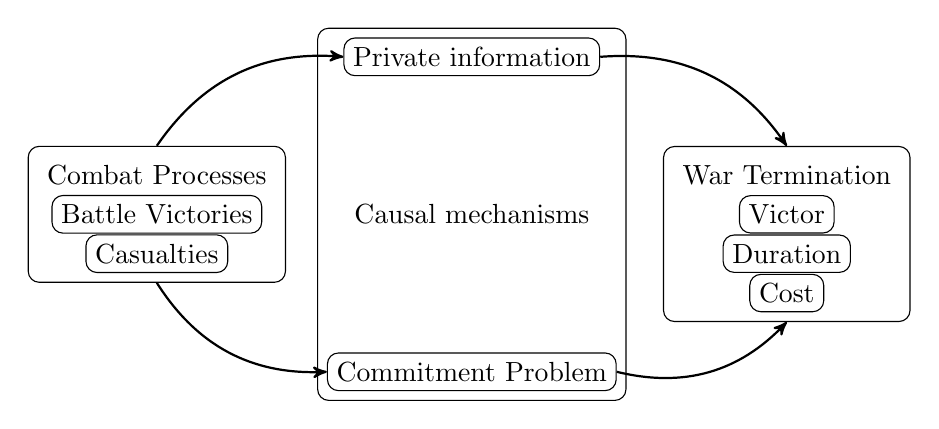
\begin{tikzpicture}[node distance=1cm, auto, scale=0.9]
  % Combat processes
 \node [] (combattitle) (combattitle) {Combat Processes};
 \node [punkt, below of=combattitle, node distance=0.5cm] (victory) {Battle Victories};
 \node [punkt, below of=victory, node distance=0.5cm] (casualties) {Casualties};
 \node [draw, rounded corners, fit={(combattitle) (victory) (casualties)}] (combat) {};

 % casual mechanisms
 \node [right of=combat, node distance=4cm] (dummy) {Causal mechanisms};
 \node [punkt, above of=dummy, node distance=2cm] (pi) {Private information};
 \node [punkt, below of=dummy, node distance=2cm] (cp) {Commitment
   Problem};
 \node [draw, rectouter, fit={(dummy) (pi) (cp)}] (causal) {};

 % war termination
 \node [punkt, right of=dummy, node distance=4cm] (wvictor)
 {Victor};
 \node [punkt, below of=wvictor, node distance=0.5cm] (wduration)
 {Duration};
 \node [punkt, below of=wduration, node distance=0.5cm] (wcost)
 {Cost};
 \node [above of=wvictor, node distance=0.5cm] (wterm)  {War Termination};
 \node[draw, rectouter, fit={(wterm) (wvictor) (wduration) (wcost)}] (end) {};

 % paths
 \draw [pil] (combat.north) to [bend left] (pi.west);
 \draw[pil] (combat.south) to [bend right] (cp.west);
 \draw[pil] (pi.east) to [bend left] (end.north);
 \draw[pil] (cp.east) to [bend right] (end.south);
\end{tikzpicture}
  \caption{Combat and War Termination}
  \label{bonds:fig:combat-causal-diagram}
\end{figure}

With regard to war, identifying the channels through which combat influences the war termination is empirically quite difficult.
Almost any observable feature of military combat alters the actual state of the war, and potentially resolves a commitment problem, and also alters the beliefs of the participants about the combat process in which they are involved, and potentially resolves a private information problem.
There are a couple ways in which this effects might be identified. %
First, if the beliefs of the participants were observed, then the effects of war events on the beliefs of the participants could be measured. %
A problem with this approach is that it requires data on the beliefs of the participants, which is difficult to acquire.
Even if first-hand accounts are available, it is not clear whether these are accurate indicators of those beliefs. %
Another problem is that it is insufficient to simply observe changes in the beliefs of one participant over time, as in \textcite{Reiter2009}. %
The causal mechanism in informational theories of war is the convergence of beliefs of the belligerents to a common distribution, which requires knowing the beliefs of both sides.
Second, it could be identified if commitment problem that started the war were known and changes it were observable. 
Third, it could be identified through a structural model of how military combat influences war outcomes.
Then it may be possible to back out how belligerents would update their beliefs and how combat could result in military victory or resolve commitment problems.
However, this would require more work which focus on generating models of military combat, even if these models are not related tied to political variables.
To understand how fighting resolves the frictions in bargaining, either changes in those frictions must be observed, or it is necessary to understand the process that underlies the fighting. %
One  difficulty in the later is that  military combat may be extremely heterogeneous, both across time and space \parencite{Reiter2003}.
But that is not a reason to ignore the study of military combat, but a call to describe and explain those patterns.
A better understanding of the the military combat process in war may have different implications for these models, and improve the ability to distinguish between these causal mechanisms.%
\footnote{%
  For example, \textcite{Walter2009} conjectures that insurgency is slower to reveal information than other forms of war. %
  Rigorously evaluating theories in this manner would require better theories of the actual military rationale between insurgency versus conventional war, the characteristics of each, and when belligerents choose to use each.
}



\section{Why The American Civil War?}
\label{sec:why-american-civil}

The American Civil War is a war with plentiful, and high quality battle-level data, and in which there are financial assets which proxy expected war outcomes well.
In terms of its battle data, the American Civil War is one of the best documented wars, so quality battle-level is available.%
\footnote{%
  For example, \textit{The Official Records of the Union and  Confederate Armies} \parencites{US1901}, published between 1880 and 1901, consists of 128 books in 70 volumes totaling 139 thousand pages.

} %
In Section~\ref{sec:why-prices-study}, I discuss why financial assets issued by the belligerents of the American Civil War may be good proxies for its war outcome.

Like any case, its generalizability is limited by its similarity to other observations.
But despite its age, the American Civil War has several similarities to contemporary civil wars.
First, the American Civil War is, if not the first modern war, a wars in the transition to modern warfare.
This war introduced several of the technologies which came to prominence in World War I and later wars: rifled artillery, telegraph, machine guns, barbed wire, ironclad warships, and submarines \parencites[89][]{Fuller1956a}[760]{Weiss1966}.
Second, the American Civil War was primarily a conventional war.
This places it in the plurality of post-Cold War civil wars, which are more often conventional wars than insurgencies \parencite[423]{kalyvas2010inter}. %
Finally, by the Civil War was U.S. was industrializing and the purchasing power parity adjusted GDP per capita of the U.S. and Confederate States in 1860 would classify them them as lower-middle income countries today.%
\footnote{%
  The GDP per capita of the US in 1860 was \$2,241 in 1990 GK international dollars. %
  In 2010, Cambodia had a GDP per capita of \$2,450, Pakistan \$2,494, and Ghana \$1,922 \parencite{BoltZanden2013}. %
  The southern states were poorer than the northern states, with a per capita consumption of about 70 percent of the overall U.S. level \parencite[324]{GoldinLewis1975}.
  The GDP per capita of the pre-war Confederacy is similar to that of Angola, Iraq and Senegal in 2010.%
  The estimated GDP per capita of the southern states in 1860 at 70\% that of the northern states was \$1,568. %
  In 2010, the following countries had approximately the same real GDP per capita: Angola \$1,600, Iraq \$1,610, and Senegal \$1,507 \parencite{BoltZanden2013}. %
}

The American Civil War is also an interesting case for study in its own right.
Its importance to American history is obvious, and need not be stated.%
\footnote{See \textcite{McPherson2003} among too many others to list.}
But, given the voluminous literature on the subject, it is surprisingly understudied in at least two regards. %
First, the international relations literature has largely ignored this conflict.
While the inter-state war literature considers it a civil war, and the civil war literature focuses on the post-1945 era \parencites[140-141]{Reiter2009}[2]{Poast2012}. %
Exceptions to this are \textcite{Reiter2009} and \textcite{Poast2012}.
Second, almost none of the existing work on the American Civil War conflict, including the few examples in international relations, use quantitative methodologies. %
\footnote{\textcite{Weiss1966} for an example from operations research.}
In applying international relations theory and quantitative methods to the study of this war, this work contributes a droplet to the ocean that is the literature on the American Civil War.



\section{U.S. Government Bond Yield Data}
\label{sec:why-prices-study}



\subsection{The Fives of 1874}
\label{sec:5s-1874}

I use the yields of long-run U.S. government bonds as a measure of the expected outcome of the American Civil War.
While the yields U.S. government bonds almost certainly were primarily driven by war expectations, they were plausibly influenced by both expectations of U.S. victory and expectations of war costs.
However, it is likely that the expectations of war costs is the more prominent of those factors.
In this work, I use the the yields of the Fives of 1874, a U.S. government coupon bond.
It is the only U.S. government bond that was both issued prior to the war and quoted throughout the war, meaning that it is the only time series of a single asset that spans the war.

The Fives of 1874 were a coupon bond authorized by the Act of June 14, 1858 to pay for a budget deficit due to the Panic of 1857, a financial panic and recession.%
\footnote{
  See \textcites[p. 76]{Bayley1882}[78--79]{DeKnight1900}[42-43]{Treasury1863}[300-301, 305]{HomerSylla2005}.
}
As their name suggests, the Fives of 1874 were a coupon bond with a coupon rate of 5 percent per-annum paid semi-annually, and redeemable in 1874.
Thus, during the period considered here, 1861--1865, the Fives had a maturity of 13--9 years.
Like most U.S. government bonds in this period, the Fives of 1874 paid interest and principal in specie (gold dollars).
They continued to pay interest in specie even after the U.S. Treasury ceased the redemption of Greenbacks, U.S. non-interest bearing notes used as currency issued during the war, in gold.\footnote{
  U.S. currency floated against the gold dollar from January 1st, 1862 until the resumption of convertibility on January 1st, 1879 \parencites{Mitchell1908}{Dewey1918}{WillardGuinnaneEtAl1996}.
}

Data on the prices of the Fives of 1874 come from tables in the two leading monthly financial magazines of the era, the \textit{Bankers' Magazine and Statistical Register} and the \textit{The Merchants' Magazine and Commercial Chronicle} \parencites[186]{Mitchell1903}.
In these publications, and in this era, the prices, not the yields, of bonds were quoted.
The prices were quoted in currency, and not in gold dollars, even though they paid interest in gold dollars.
I converted the prices to gold dollars using the current exchange rate of Greenbacks to gold dollars in New York, using the \textcite{Mitchell1908} data.%
\footnote{
  Available in digital form at \url{http://eh.net/wp-content/uploads/2013/11/greenback.txt} from \textcite{WillardGuinnaneEtAl1996}.
  I made some corrections to it where there were incorrect transcriptions from the original source.
}
The yields of the bonds were calculated by converting prices to gold dollars accounting for the current exchange rate and the expected depreciation of the gold dollar.%
\footnote{
  Since the price of bonds was quoted in currency but it paid interest and principal in currency, calculating the yields is difficult since they also incorporated beliefs about the future prices of gold dollars \parencites[Appendix A]{Macaulay1938}{Roll1972}{Calomiris1988}[302-303]{HomerSylla2005}.
  Most bonds, including the Fives of 1874, were priced in U.S. currency but paid specie and often principal in gold dollars.
  This work accounts for this using a simple method to calculate the future price path of the dollar; it assumes that currency with appreciate at the risk free interest rate of 5 percent until it reaches parity with a gold dollar.
  This follows from an assumption that the risk free rate is constant over the period, and the gold dollar is priced as a risk-free zero-coupon bond with an unknown redemption date \cite{McCandless1996}.
  \textcite{Roll1972} and \textcite{Calomiris1988} estimate the expected depreciation of gold dollars in Greenbacks using differentials in bonds, however those methods cannot be applied to the period considered here.
}
Calculating the price and yield in gold dollars rather than currency is a meaningful decision, because while the price and yield in gold dollars fluctuated throughout the war, the price and yield in currency were stable.%
\footnote{See \textcite{Roll1972} for an analysis of this phenomena.}
This suggests that investors were less worried about a complete default than an implicit default in which government would redeem interest or principal payments in depreciated currency rather than specie.
Both sources quote the bonds at irregular, but approximately weekly frequencies.
\footnote{\textit{Bankers' Magazine}: 3--15 days, with a median of 10 days; \textit{Merchants' Magazine}: 4--23 days, with a median of 7 days.}
For the analysis, data from these two sources are combined to form a single series.

I collected and provide the raw financial data used in this work, as well as additional financial and economic from the American Civil War period in the American Civil War Era Financial Data Collection (ACWFD) \parencite{Arnold2015a}.%
\footnote{Also available at The dataset is at \url{http://github.com/jrnold/civil_war_era_findata}.}
This data collection contains bond prices and exchange rates published in the \textit{Bankers' Magazine} and \textit{Merchants' Magazine}, bid-level auction data for U.S. government bond auctions, and miscellaneous financial and economic data for this period from a variety of primary and secondary sources.

Figures~\ref{bonds:fig:fives1874_price} and~\ref{bonds:fig:fives1874_yield} plot the price in gold dollars and the yield to maturity of the Fives of 1874.
Prior to mid-1860, the yield of the Fives was low with little variation, fluctuating between 4.5 and 5 percent.%
\footnote{
  This is actually below was generally considered risk-free rate in the U.S. for that period, 5 percent, which \textcite[29]{Elder1863} calls the ``natural rate of interest on [government] Loans''.
  During this period British 3 percent consols had a yield of between of 3.10 and 3.28 \parencite[193]{HomerSylla2005}.
}
After Lincoln's election in November 1860,  the interest rate rose to 6 percent.
After the initiation of the war with the Battle of Sumter (April 12--14, 1861), the yield rose to 8.2 percent.
During the war, between April 1861 and April 1865, the yield fluctuated between 5.2 and 14.7 percent, reaching its peak on July 30, 1864.
After the end of conflict in April 1865, the interest rate returned to stability at 6.5 percent, a rate higher than its pre-war level.


The Fives of 1874 were one of several bonds issued by the U.S. government during this period, but it has several advantages over other bonds for the purpose of this analysis.
The Fives of 1874 were the only coupon bond regularly quoted for the entire war, April 1861--May 1865, in the sources considered here.
The reason it is the only such bond, is that while the U.S. issued much debt during the Civil War, it had little debt in the antebellum period, and thus there were few outstanding bond issues at the start of the war.
\footnote{
  After paying off the debt issued during the War of 1812, the U.S. government had no outstanding debt between 1835 and 1842 \parencite[297]{HomerSylla2005}.
  The debt as a percentage of GDP rose from 1.9 percent in 1860, before the war, to 31.4 percent in 1866, its peak just after the war \parencites{CBO2012}{CBO2012a}.
}
The only other bond was widely traded at the start of the war, was the Sixes of 1868.
However, \textit{Bankers' Magazine} stops quoting the Sixes of 1868 in September 1861.
Another bond, the  Sixes of 1881 were issued under acts in February and July 1861, just prior to and just after the start of the war, but they are not regularly quoted in the \textit{Bankers' Magazine} until September 1861, five months after the start of the war.
The U.S. issued several other bonds of various maturities and rates throughout the war, but they provide even shorter time series.
In many cases these loans are exotic relative to government debt issues today.
Some contained options to exchange the bond for other bond issues or were callable by the government. 
Both of these make it difficult to calculate the yields for these bonds.
\footnote{
  The 5-20's and 10-40's were bonds callable by the government after 5 (10) years and redeemable in 20 (40) years.
  The 7-30's were bonds that had coupon rates of 7.30 percent (2 cents per day), were redeemable in 3 years, but included the option to be exchanged for either the Sixes of 1881 or 5-20's.
  See \textcites{Bayley1882}{DeKnight1900}[297--309]{HomerSylla2005} for overviews of U.S. debt issues during this period.
}
Using the Fives of 1874 instead of these other bonds does not make a substantive difference, since as Figure~\ref{bonds:fig:fives1874_union} shows, the patterns of the yield to maturity of the Fives of 1874 is similar to the yields of all the other bonds issued by the U.S. government.
\textcites{WillardGuinnaneEtAl1996}{McCandless1996}{SmithSmith1997} use the exchange rate of Greenbacks to gold dollars in their analyses.
However, since the U.S. did not issue Greenbacks until after the start of the war, and did not suspend the redemption of that currency for gold until January 1, 1862, any analysis using only Greenback prices cannot cover the first eight months of the war, April--December 1861.
This is the period which should have the highest informational content in an informational theory of war, and includes battles such as the First Battle of Bull Run, and the Battle of Wilson's Creek.%
\footnote{\textcite{Poast2012} argues that the First Battle of Bull Run was pivotal in avoiding British recognition of the Confederate States.}
Apart from the loss of observations, using Greenbacks instead of the Fives of 1874 would not make a substantive difference, since as Figure~\ref{bonds:fig:fives1874_greenbacks} shows, the price of Fives of 1874 in gold dollars is similar in both level and trend as the the price of Greenbacks in gold dollars.

The American Civil War is an ideal case in which to use prices to infer expectations of war termination for three reasons.
First, The war was of such severity that the nearly the entire budget of the U.S. government was war-related military spending, and thus fiscal expectations corresponded to military spending expectations. %
For the U.S., the War and Navy Departments accounted for 76 percent (in 1862) to 61 percent (in 1865) of the expenditures.
The fraction of the budget spent directly on the military by the Union fell over the course the war as the fraction spent on paying the principal and interest on its debt, increased from 20 (1862) to 36 (1865) percent of the budget.
The overwhelming the majority of that debt had been issued to fund the war \parencites{Treasury1861a}{Treasury1861b}{Treasury1862}{Treasury1863}{Treasury1864}{Treasury1865}, so payments on debt serving were themselves simply delayed military spending.
As \textcite[][668]{McCandless1996} states, ``[d]uring the war, the single most important indicator of future government expenditures is the process of the war itself.''
% INSERT FIGURE OF THE BUDGET

Second, there is extensive economic history literature establishing that war events are the single best determinant of bond and currency prices during the American Civil War:
\parencites{Mitchell1903}{Mitchell1908}{Calomiris1988}{WillardGuinnaneEtAl1996}{McCandless1996}{SmithSmith1997}, graybacks \parencites{Schwab1901}{Weidenmier2002}, southern prices
\parencite{BurdekinLangdana1993}, Confederate bonds \parencites{DavisPecquet1990}{BrownBurdekin2000}{OosterlinckWeidenmier2007}, and Union bonds \parencite{Roll1972}.%
\footnote{One notable exception is \textcite{BurdekinWeidenmier2001}, which shows that the prices of graybacks in Richmond and Houston diverged due to differential application of monetary reform in late 1864.}
%These are largely interested in showing that the markets efficiently responded to new information in the war; this work is inverting that, and starting with the assumption that the markets are efficiently processing new information to understand imporant

Third, statements by and the actions of contemporary investors indicated the importance that war events had on the prices. %
Members of the government, military, and reporters all engaged in investment speculation based on their knowledge of war events \parencites[5-7]{Cornwallis1879}{Mitchell1903}[][1004]{WillardGuinnaneEtAl1996}.
Investment firms even had their own correspondents stationed in cities close to the war fronts to relay the latest news \parencites[5-7]{Cornwallis1879}. %
Finally, magazines and newspapers often cited war events as the cause of recent price movements. %
For example, the issue of \textit{Bankers' Magazine} after Gettysburg and Vicksburg (Jul 23, 1863), cites these battles as the cause of the recent changes in market prices,
=\begin{quote}
  The month of July has been a very active one with numerous fluctuations, almost daily, in the market values of gold, with unusual changes in the current values of stocks. %
  The advices as to the war movements are of a most satisfactory kind, leading to a fall in gold from 146 1/2 at the close of June, to 123 1/2, the 20th inst., at which dates the public had learned the  capitulation of Vicksburgh and of Port Hudson, the defeat of Lee in  Maryland and Pennsylvania, and of successful results at other points  for the Union forces. %
\parencite[159]{BankersMagazine1864}
\end{quote}



\subsection{U.S. Government Bond Yields are Primarily a Function of the Expected Cost of the War}
\label{sec:u.s.-governm-inter}

Since the cash flows of U.S. government bonds are not directly related to a war outcome, in order to treat those yields as an expectation of a war outcome, I need to, first, establish which war outcomes can influence future cash flows, and, second, establish that expectations about war outcomes are the primary factor influencing the yield.
The U.S. government bond yields are plausibly related to both expectations about whether the U.S. would win the war, as well as the cost of the war to the U.S. government.
These two expectations have possibly cross-cutting implications on bond yields.
An increasing probability of U.S.\ victory would have a would make bonds less risky, a higher price and lower yield, while a increasing expectation of war cost would make bonds more risky, a lower price and a higher yield.
Unfortunately, it is not possible to separate these effects using only U.S. government bond yield data.
However, it is likely that U.S.\ government bond bond yields mostly responded to expectations about war costs, and can be considered a proxy for the expected cost of the war for the U.S.

The risk on U.S. government bonds depended on the war cost for several reasons.
The  war was funded primarily through debt, and thus, expectations of a longer or more vigorously fought war almost directly implied an increase in government debt.
The proportions of the U.S. government revenues for each source of funding as follows: taxes 72--89\% from loans, 11--25\% from taxes, and 0--4\% from miscellaneous sources (tariffs, land sales).
In its analysis of the future fiscal situation, the 1863 \textit{Annual Report of the Treasury} notes that taxes and other revenue sources were covering the non-war expenses and debt payments in its budget, but new debt was being issued to pay for the military expenditures needed to wage the war \parencite[10-13]{Treasury1863}.
\footnote{See also \textcite[][14]{Godfrey1976}.}
The budgetary effect of the war is clear from  comparing forecasts of the U.S. budget for the 1866 fiscal year made before and after the war had ended.
In \textit{The Annual Report of the  Treasury} issued on December 6, 1864 the forecast deficit for FY 1866, assuming that the continued, was \$470 million, with \$1,168 million in expenditures \parencite[13]{Treasury1864}.
In the following year's \textit{Annual Report}, issued in December, 1865, after the conclusion of the war, the Treasury estimated a surplus of \$112 million, with expenditures of only \$396 million dollars \parencite{Treasury1865}.
This forecast was close to what would be the actual surplus, \$132 million \parencite[2]{Treasury1866}.
Thus, both expectations of the government military expenditures and the length of the war should have had a direct impacts on investors' expectations of the eventual debt level of the U.S. government.
This increased debt would increase the possibility of default or the temptation of the government to repay its debt in currency rather than specie.

The future resources of the U.S. to pay off that debt also depended on the result of the war, namely, whether the seceding states would be reincorporated into the U.S. and potentially help pay for the costs incurred in the war.
The size and wealth of the seceding Southern states was much smaller than those of the Northern and Western states.
In 1860, the states that would make up the Confederacy accounted for 29 percent of the overall U.S. population,%
\footnote{
  Southern states included VA, TN, GA, NC, AL, MS, LA, SC, TX, AR, FL \textcite[5]{Eicher2001}.
  Wealth is used instead of GDP, since GDP was not calculated until after WWI, the total wealth of individuals, as reported in the Census is a better measure of what contemporaries knew.
}
and 25 percent of the total wealth.%
\footnote{
  \textcite[12]{Elder1865}. Wealth is defined as the value personal property excluding slaves, which was asked on the 1860 Census.
  It may be a better measure of how contemporaries would have viewed the value of the South than GDP because GDP had not yet been invented.
  The closest contemporaries had to GDP was an approximation that the value of yearly production was about 25-27 percent of total wealth \parencites[7]{Elder1865}[24]{Treasury1865}.
}
% TODO: What was the Confederacy GDP?

Some statements by government officials and market participants suggest that they were more concerned with the cost and duration of the war than with the the reincorporation of the seceding states.
William Elder, a leading economist of the era, in an 1863 analysis of the ability of the U.S. to repay its debt, stated ``The Rebellion leaves our capital in real and personal property just where it was before the secession. \dots{} So far now this is only a loss of that which we have not had, and at best or worst, a very small one in any time of need'' \parencite[19]{Elder1863}.%
\footnote{
  However, \textcite{Elder1863} does emphasize the importance of the resources of the Western territories, which perhaps strengthens the argument of  \textcite{Weingast1998} that he U.S. was concerned that Southern states seceding could lead to Western states seceding.
}
The \textit{Annual Report of the Treasury Department} in 1863 highlighted this relationship between cost of the war and the interest rate it paid on its bonds:
\begin{quote}
It will not escape observation that the average [interest] rate is now increasing, and it is obvious that it must continue to increase with the increase of the proportion of the interest-bearing to the non-interest-bearing debt.
And as the amount of the latter, consisting of United States notes and fractional currency, cannot be materially augmented without evil consequences of the most serious character, the rate of interest must increase with the debt, and approach continually the highest average.
That must be greater or less in proportion to the duration and cost of the war. \parencite[13]{Treasury1863}
\end{quote}

The striking difference in the trend of the prices of U.S. bonds and that of the Confederate currency (Graybacks) in Figure~\ref{bonds:fig:fives1874_compared} is also evidence that U.S. bond yields were less driven by expectations of U.S. victory than by the war cost.
That figure shows that the price of the Confederate currency (Graybacks) in terms of gold dollars decreases almost monotonically over the entire course of the war.
Although the price of Graybacks is partially determined by the money supply \parencite{BurdekinWeidenmier2001}, the price of Confederate bonds issued in Amsterdam and payable in gold followed a similar pattern, decreasing nearly monotonically from mid-1863 onward \parencite{HaberMitchenerOosterlinckEtAl2015}.
The prices of the Confederate assets were likely primarily determined by whether the U.S. would win the war and repudiate their debt \parencite{HaberMitchenerOosterlinckEtAl2015}.
If the U.S. bonds primarily reflected the probability of U.S. victory, then the expected trend of its prices (yields) would increase (decrease) immediately after the start of the war, and almost monotonically increase (decrease) throughout the war, or at least from mid-1863 onward.
However, Figure~\ref{bonds:fig:fives1874_yield} shows that while the yields of U.S. government bonds fluctuate early in the war, they do not decrease over the course of the war.
Instead, they spike in mid-1864 at a point at which U.S. victory should have been highly probable if not almost certain.
This suggests that U.S. government bond yields do not primarily reflecting expectations of U.S. victory, and are, instead, reflecting some other factor, which is likely war costs.

Finally, the financial benefit of victory to the U.S. and the war costs are inversely related.
The longer and more destructive the war, the less the ability of the Southern states to provide for the repayment of the debt incurred by the U.S. in fighting the war.
In fact, immediately after the war, the U.S. government attempted to collect direct taxes from the Southern states, but it soon suspended that collection after it became clear that the Southern states could not pay them.
Treasury Secretary Hugh McCullough justified this suspension by noting that the inhabitants of the Southern states ``had been subject to heavy taxation by the government which was attempted to be established in opposition to that of the United States, and had been greatly exhausted by the ravages of war.'' \parencite[29]{Treasury1865}.
In analyses of the repayment of debt after the war by the Treasury Department and others \parencites{Elder1865}{Treasury1865}{Walker1865a}, the wealth of the Confederate states was assumed to remain constant between 1860 and 1870 due to the destruction of the war, and that they would not be able to contribute to the repayment of the debt until after 1870.

% todo: longer war reduced the pie. Confederacy in worse shape to repay the debt. E.g. ability to extract a direct tax.

While the precise meaning of the bond yields in terms of a war outcome is unclear, it is clear that the bond yields almost completely reflect war expectations.
As noted earlier in this section, military expenses accounted for the overwhelming majority of U.S. government expenditures between 1861 and 1865, so there are no other budgetary concerns that could plausibly have been affecting investor's expectations.
The importance of the war is also clear from comparing the level and variance of U.S. government bond yields during the war with the preceding period.
During 1856--1860 yields on U.S. government bonds were stable at below 5 percent.
At the height of the the Panic of 1857, the yield of U.S. government bonds (Sixes of 1868) only reached 5.1 percent.%
\footnote{Data from the \textit{Bankers' Magazine} and the author's calculations. Also see \textcite{HomerSylla2005}.}
Since a major financial crisis had little effect on bond yields prior to the war, there are certainly no non-war omitted factors affecting the yields.
This is not to say that the battles in the war are the only factor affecting the bond yields.
Government policies, elections, and other events could and almost certainly did have some affect on bond yields.
But all of these other events were affecting government bond yields through their effects on investors' expectations of the war.

In summary, the U.S. government bond yields reflected some combination of expectations about the cost and the victor of the war, weighted by how each of these would affect the ability of the U.S. government to repay its debts.
However, it is more likely that these yields are largely reflecting expectations about the cost and duration of the war.

\begin{figure}[!htpb]
  \centering
  \begin{subfigure}[b]{\linewidth}
   \includegraphics{../bonds_and_battles//paper/figure/fives1874_price-1}
  \caption{Price in gold dollars. Par value is \$100.}
  \label{bonds:fig:fives1874_price}
\end{subfigure}
\begin{subfigure}[b]{\linewidth}
   \includegraphics{../bonds_and_battles//paper/figure/fives1874_yield-1}
  \caption{Yield to maturity.}
  \label{bonds:fig:fives1874_yield}
\end{subfigure}
\caption[Price and yield of the Fives of 1874, 1858-1865]{Price and yield of the Fives of 1874 from its issue in 1858 until the end of the Civil War in 1865.
The yield is steady at near 5 percent until the election of Lincoln and the secession of the Southern States in late 1860-early 1861.
During the American Civil War, the yields are variable, spiking in the middle of 1864.
 }
\label{bonds:fig:fives1874_yield_price}
\end{figure}

\begin{figure}[!htpb]
  \begin{subfigure}[b]{0.45\linewidth}
    \includegraphics{../bonds_and_battles//paper/figure/fives1874_greenback_price-1}
  \caption{Price in gold dollars for the Fives of 1874 compared to the price of Greenbacks, 1862-1865.}
  \label{bonds:fig:fives1874_greenbacks}
\end{subfigure}%
\hspace{0.1\linewidth}%
\begin{subfigure}[b]{0.45\linewidth}
    \includegraphics{../bonds_and_battles//paper/figure/fives1874_union-1}
    \caption{Yield to maturity of the Fives of 1874 compared with other U.S. bonds.}
  \label{bonds:fig:fives1874_union}
\end{subfigure}

%% \begin{subfigure}[b]{0.45\linewidth}
%%   \centering
%%   \includegraphics{file.path(fig_path, "fives1874_north-1")}
%% \caption{Yield to maturity of the Fives of 1874 compared with bonds issued by Northern states.}
%% \label{bonds:fig:fives1874_north}
%% \end{subfigure}%
%% \hspace{0.1\linewidth}%
%% \begin{subfigure}[b]{0.45\linewidth}
%%   \includegraphics{file.path(fig_path, "fives1874_south-1")}
%% \caption{Yield to maturity of the Fives of 1874 compared with bonds issued by Southern and border states.}
%% \label{bonds:fig:fives1874_south}
%% \end{subfigure}

\begin{subfigure}[b]{0.45\linewidth}
  \includegraphics{../bonds_and_battles//paper/figure/fives1874_graybacks-1}
\caption{Price in gold dollars of the Fives of 1874 compared with \$100 Graybacks (Confederate currency).}
\label{bonds:fig:fives1874_grayback}
\end{subfigure}
\caption[The Fives of 1874 compared with other government and states issued bonds and currency.]{The Fives of 1874 compared with other government and states issued bonds and currency.
  The Fives of 1874 follow a similar pattern as that of other U.S. bonds and those issued by Northern states.
  They diverge and have a different pattern than the Confederate currency and bonds issued by Southern states.
}
\label{bonds:fig:fives1874_compared}
\end{figure}

% TODO: this needs qualitative overview of the


\section{Battle Data}
\label{sec:battle-data}

A theoretical and practical issue in the empirical study of war is how to operationalize military combat within wars.%
\footnote{
  See the discussions in \textcites{ReiterStam1998}{BiddleLong2004}{Reiter2003}{GrauerHorowitz2012}{Weisiger2015}.
}
There are two major issues in the operationalization of military combat.
The first is ``what the unit of observation?''
Some work uses events, \eg{}battles or campaigns, as the unit of observation \parencites{ReiterStam1998}{ReiterStam2002}{Ramsay2008}[59-60]{Reiter2009}{PilsterBoehmelt2011a}{GrauerHorowitz2012}, while other work uses time-period aggregated values, \eg{}monthly casualties \textcite{Weisiger2015}.
The second is ``how to measure military success?''
Some work uses victory or defeat in battle \parencites{ReiterStam1998}{ReiterStam2002}{GrauerHorowitz2012}, while other work uses casualty-based measures, such as loss-exchange ratios  \parencites{Biddle2004}{BiddleLong2004}{PilsterBoehmelt2011a}.
In this work, I quantify military combat in the American Civil War by focusing my analysis on a set of important battles, and define success in combat by victory in battle, \ie{}Union or Confederate victory.
An advantage of this method is that it allows me to estimate effects for individual battles with fewer assumptions of how features of those battles relate to war outcomes, and as well as the average effect of Union and Confederate battle victories.

The battles used in this analysis are listed in Table~\ref{bonds:tab:battles}.
This is the set of battles which the National Park Service's Civil War Sites Advisory Commission (CWSAC) classified as the most important in the war \parencite{CWSAC1993}.
These data come from the 1993 CWSAC report, \textit{Civil War Sites Advisory Commission Report on the Nation's Civil War Battlefields} \parencites{CWSAC1993}{CWSAC1993b}.
The CWSAC was a commission established in accordance with a 1990 law to preserve Civil War battlefields and was ``asked to identify the nation's historically significant Civil War sites; determine their relative importance; determine their condition; assess threats to their integrity; and recommend alternatives for preserving and interpreting them.'' \parencite{CWSAC1993b}
As part of that process they identified 383 battles, of the over 10,500 military engagements listed in the \textit{Official Records of the American Civil War}, as the ``principal battles'' of the war based on a ``military significance'' criteria.
As to the comprehensiveness of their list, \parencite{CWSAC1993} states,
\begin{quote}
  These [battle] sites encompass virtually all of the principal land battles that were of special strategic, tactical, or thematic importance to local operations, campaigns, theaters, or to the war as a whole \dots{}
  The more than 10,500 conflict sites excluded from our inventory were relatively unimportant as individual military actions.
  These conflicts were the venues and actions that implemented the war between and beyond the dramatic major engagements.
\end{quote}
These principal battles were further classified into four categories of military significance: ``A'', ``having a decisive influence on a campaign and a direct impact on the course of the war'', to ``D'', ``having a limited influence on the outcome of their campaign or operation but achieving or affecting important local objectives''.
This work uses 43 battles with the ``A'' military significance classification.%
\footnote{
  Three CWSAC class ``A'' battles are omitted from the analysis.
  The Battle of Fort Sumter (SC, April 12--14, 1861) is omitted because it marks the start of the war and the analysis starts after this battle.
  Given the small size of Fort Sumter, no casualties, the effects of the battle can be attributed to marking the start of conflict.
  The Battle of Fort Blakely (AL, April 2--9, 1865) is omitted because news of battle does not reach New York City until after news of the surrender of Gen. Robert E. Lee's forces at Appomattox Court House on Apr 10, 1865.
  The Battle of Five Forks (VA, April 1, 1865) is omitted because I could not find reports of it in the \textit{New York Times}; news of it was overshadowed by the Third Battle of Petersburg on April 2nd, which ended the Siege of Petersburg and started the Appomattox Campaign, which ended in the surrender of Robert E. Lee.
}
While this is a subset of the battles in the American Civil War, it is still a relatively large number of battles by most war standards and similar in number and composition as the list of battles provided by other sources.
\textcite{Livermore1900} includes 63 battles, \textcite{Bodart1908} includes 50, and \textcite{cdb90} includes 49.
That this set of battles is a subset of battles in the  American Civil War is largely due to the completeness of the records and richness of the data on the American Civil War.

\begin{figure}[!htpb]
  \centering
  \includegraphics{../bonds_and_battles//paper/figure/fig_major_battles-1}
  \caption{Major battles and their outcomes}
  \label{bonds:fig:major_battles}
\end{figure}

The CWSAC report \parencite{CWSAC1993b} assigns a result to each battle, which is one of ``Union victory'', ``Confederate victory'', or ``Inconclusive''.
While \textcite{CWSAC1993} does not explicitly describe the methodology used to classify the battle outcomes, the classifications largely agree with other sources \parencites{fox1898regimental}{Livermore1900}{Bodart1908}{cdb90}, several of which are themselves cited as sources of the report.
Two of those sources, \textcite{fox1898regimental} and \textcite{Livermore1900}, provide more description of how they assigning the winner of a battle.
Generally, the victorious side of a battle is considered to be the side that controls the battlefield at the end of battle.
The data used in this work includes 30 Union victories, 13 Confederate victories, and no ``Inconclusive'' battles.
\footnote{
  In the original CWSAC data, there were two ``Inconclusive'' battles: The Wilderness, and Spotsylvania Court House.
  In the analysis, these were recoded as a Union victory and a Confederate victory, respectively, since with only two battles, I cannot estimate an average effect of ``Inconclusive'' battles.
  The Wilderness was reclassified as a Union victory, and Spotsylvania Court House as a Confederate victory based on how the results were reported in the \textit{New York Times}.
}
Figure~\ref{bonds:fig:major_battles} plots the date and outcomes of these battles over time.
In the analysis, I will not explicitly include casualty or force size data.
By selecting on the most militarily significant battles, I have already effectively selected those battles with the highest casualties and force sizes.

\begin{table}
  \centering
  \input{../bonds_and_battles//paper/tex/tab_major_battles.tex}
  \caption{List of the 43 major battles of the American Civil War included in this analysis.}
  \label{bonds:tab:battles}
\end{table}

In order to estimate the effects of these battles on bond yields, I also need the days on which the New York markets received news about these battles.
These is not the same as the dates of the battle, because news reaches the market with a lag.
In general, New York markets received news about battles surprisingly quickly:
\begin{quote}
Members of both Houses [of Congress], and of all political creeds, resident bankers, the lobby agents, clerks, and secretaries, haunted the War Department for the latest news from the seat of war.
The daily registry of the Gold Room was a quicker messenger of successes or defeats than the tardier telegrams of the Associated Press. A private secretary of a high official, with no capital at all save his position, which gave him authentic information of every shaping of the chess game of war a full twenty hours in advance of the public, simply flashed the words ``sell, buy'' across the wires, and trusted to the honor of his broker for the rest. \parencite[245]{Medbery1870a}\footnote{Originally quoted in \textcite{WillardGuinnaneEtAl1996}.}
\end{quote}
However, there was still a lag between the occurrence of the battle, and when news of the outcome reached the market.
More importantly for the analysis, this lag varied with the distance of the battle from New York and Washington, as well as idiosyncratic reasons.
For example, the market knew nothing of Sherman's army after he moved north from Savannah until he arrived in  \textcite[204]{Mitchell1903}.
As a measure of when information of the battle reaches the New York market, I coded when news about a battle was first reported in the \textit{New York Times}.
While battles the Eastern theater were often reported on the same or next day (Antietam, Gettysburg), news on battles in other theaters may not reach the market for days.
The battle with the longest lag in news was the Battle of Glorietta Pass in New Mexico; it ended on March 28, 1862, but news of the battle did not reach New York city until April 15.
For some battles which lasted several days of approximately equal intensity  (Chattanooga), I coded news as reaching the market on several days.
For sieges which could last many days, \eg{}Vicksburg, Port Hudson, I only coded when the news of the end of the siege was reported.
A data driven approach to identifying the timing of this news is important since in a time series analysis, the timing of the events is the primary factor in identifying their effects.%
\footnote{
  Measurement error due to how these dates are coded will be mitigated somewhat since prices are not observed daily, so usually the change in prices reflects the sum of the effects of several days.
}
% Illustrative anecdotes: McClellan in Peninsula campaign, Sherman in march to the sea.

In using a small set of battles based on a \textit{ex post} expert assessment of their military importance, it is important to note that this is not selecting on the dependent variable.
In this case, that would be including explanatory variables by selecting periods of times that had large changes in yields.
Instead, I am selecting a set of covariates, \ie{}battles, which are expected to have large effects on the response variable based on prior information.
This is no different than any other regression model, in which the researcher selects a relatively small set of covariates of all possible variables in the universe, because those covariates are \textit{a priori} expected to plausibly have an effect on the response variable.

For this project, I created a public data collection of American Civil War battles, the American Civil War Battle Database (ACWBD) \parencite{Arnold2015b}.%
\footnote{The data and source code of the data collection are available from \url{https://github.com/jrnold/acw_battle_data}.}
The ACWBD combines, cleans, cross-references battle data from multiple primary and secondary sources, including \textcites{Phisterer1883}{Livermore1900}{Bodart1908}{dyer1908_war_rebel}{KennedyConservation1998}{CWSAC1993}{cwsac2012}.
It is the most complete, machine-readable data on American Civil War battles of which I am aware.



\section{Statistical Models of the Effects of Battles on Bond Yields}
\label{sec:model-war-events}

In this section, I present several models of the effects of battles on U.S. government bond yields.
In all these models, the response variable is the yields of the Fives of 1875, as discussed in Section \ref{sec:5s-1874}.
The data on the Fives consist of  observations between 1861-04-27, the first observation after the Battle of Fort Sumter and the official start of the war, and 1865-05-04, the end of the month after Robert E. Lee surrendered after the Battle of Appomattox Court House.
These are observed at irregular frequencies, between 1 and 1 days, but the estimated models handles missing values without additional adjustments.
In these models, I use the logarithm of the yield since Figure \ref{bonds:fig:fives1874_yield_price} suggests that the variance of yields is increasing in its level.

All of these models are of the form,
\begin{align}
  \label{bonds:eq:6}
  \log y_{t} &= y^{*}_{t} + \epsilon_{t} & \epsilon_{t} &\sim \dnorm{0, \tau^{2}} & \text{if $y_t$ not missing} \\
  \label{bonds:eq:1}
  y^{*}_{t} &= y^{*}_{t - 1} + \delta_{t} + \eta_{t} & \eta_{t} &\sim \dt{5}{0, \sigma}
\end{align}
for days $t = 1, \dots, T$.
Equation~\eqref{bonds:eq:6} states that the observed log-yields consist of a latent log-yield ($y^{*}_{t})$ and measurement error ($\epsilon_{t}$).
Equation~\eqref{bonds:eq:1} states that the first difference in the latent log-yields, $y^{*}_{t} - y^{*}_{t-1}$, is the sum of $\delta_{t}$ and a mean-zero innovation, $\eta_{t}$.
The models differ in the definition of $\delta_{t}$ and this is where battle effects are included.
The innovation $\eta_{t}$ is distributed Student's $t$ to allow for large events that are unmodeled, \ie{}any non-battle events.
If $\tau^{2} = 0$, then Equations~(\ref{bonds:eq:6}) and~(\ref{bonds:eq:1}) would be equivalent to simply estimating the a model with the first difference of $\log y_{t}$ as the dependent variable.
With a non-zero $\tau$, and supposing $\eta$ was distributed normal, this model would be equivalent to an ARIMA(0, 1, 1) model in which the MA parameter is constrained to be negative \parencite[91]{PetrisPetroneEtAl2009}.

In this section, I estimate four models which differ in how $\delta_{t}$ is defined:
\begin{itemize}
\item $\Model{1}$ is benchmark model that does not include any battle effects.
\item $\Model{2}$ includes variables for Confederate and Union victories, but no individual battle effects.
\item $\Model{3}$ is like $\Model{2}$, but also includes random effects for each battle.
\item $\Model{4}$ is like $\Model{2}$, but the effects of Confederate and Union victories are smoothly varying over time.
\end{itemize}
Model $\Model{1}$ includes no battle effects, $\delta_{t} = 0$ for all $t$.
In models $\Model{2}$--$\Model{4}$, $\delta_{t}$ is non-zero and time-varying, and is a function of battle outcomes, but these models differ how the effects of the battles are modeled.
In model $\Model{2}$, $\delta_{t}$ includes the effects of Confederate and Union victories.
\begin{align}
  \label{bonds:eq:2}
  \delta_{t} &= \alpha + X_{t} \begin{bmatrix}\beta_{C} & \beta_{U}\end{bmatrix}'  \\
  X_{t, 1} &= \sum_{b \in B} W_{b,t} && \text{if $b$ is a Confederate victory} \\
  X_{t, 2} &= \sum_{b \in B} W_{b,t} && \text{if $b$ is a Union victory} \\
  W_{b,t} &= 
            \begin{cases}
              \frac{1}{n_{b}} & \text{If news of battle $b$ reached the market on day $t$.} \\
              0 & \text{otherwise}
            \end{cases}
\end{align}
where $B$ is the set of all battles in the data (Table \ref{bonds:tab:battles}).
In this model, all Confederate victories have the same effect on the yield, and all Union victories have the same effect on the yield. 
In other words, given the result, battles are exchangeable.
The parameters $\beta_{C}$ and $\beta_{U}$ are the average effects of Confederate and Union victories.
The matrix $W$ is is a $T \times |B|$ matrix, in which each column is a variable indicating if there was news about a battle reached on that day.
News of battles is assumed to reach the market on the days the first news of the battle is reported in the \textit{New York Times} and the following 5 days.
For a given battle, each day in which news is received is given an equal weight, and the weights for each battle sum to one.
$n_{b}$ is the total number of days for which news of battle $b$ reached the market.
For example, the end of Gettysburg was reported in the news on July 2nd--4th, 1863, so July 2, 1863 through July 9, 1863 have a weight of $\frac{1}{8}$, and all other days have a weight of 0.
$X_{t}$ is an $T \times 2$ matrix containing the sum of the weighted indicators of Confederate and Union victories occurring on day $t$. 
Since each column of $W_{b}$ sums to one, $\beta_{C}$ is interpreted as the average effect of a single Confederate victory, and $\beta_{U}$ as the average effect of a single Union victory.
Finally, $\alpha$ is a parameter representing a constant trend in the yields not due to the battles.

In model $\Model{3}$, $\delta$ also includes random effects for each battle,
\begin{align}
  \label{bonds:eq:10}
  \delta_{t} &= \alpha + X_{t} \begin{bmatrix}\beta_{C} & \beta_{U}\end{bmatrix}' + W_{t} \gamma' \\
  \label{bonds:eq:12}
  \gamma_{b} &\sim \dt{7}{0, \zeta^{2}}
\end{align}
where $\alpha$ and $\beta$ have the same meaning as in $\Model{2}$, and $\gamma$ is a $|B| \times 1$ row vector with random effects for each battle.
The random effects, $\gamma$, are given a Student's $t$ distribution since it is expected that a few battles will have particularly large effects.
The total effect of an individual battle is the average effect of its result plus its random effect,
\begin{align}
  \omega_{b} =
  \begin{cases}
    \beta_{C} + \gamma_{b} & \text{if $b$ is a Confederate victory} \\
    \beta_{U} + \gamma_{b} & \text{if $b$ is a Union victory}
  \end{cases}
\end{align}

In model $\Model{4}$, the effect of each battle, $\omega_{b}$, is shrunk towards both the average effect of its result and and the effect of the previous previous battle of the same result.
This is equivalent to a model in which the effects of Confederate and Union victories are smoothly time-varying with an $AR(1)$ process.%
\footnote{
   $\omega_{C,t} \sim N(\beta_{t,C}, \zeta^{2}) N(\omega_{C,t-1}, \xi^{2}) = N((1 - \rho) \beta_{C} + \rho \omega_{C,t-1}, \rho \zeta^{2})$, where $\rho = \frac{\xi^{2}}{\xi^{2} + \zeta^{2}}$.
}
\begin{align}
  \label{bonds:eq:11}
  \delta_{t} &= \alpha + W_{C,t} \omega_{C} + W_{U,t} \omega_{U} \\
  \omega_{C,b} & \sim \dnorm{(1 - \rho) \beta_{C} + \rho \omega_{C,b-1}, \rho \zeta^{2}} & \text{for $b \in \{2, \dots, C\}$} \\
  \omega_{C,1} & \sim \dnorm{ \beta_{C}, \zeta^{2}} \\
  \omega_{U,b} & \sim \dnorm{(1 - \rho) \beta_{U} + \rho \omega_{U,b-1}, \rho \zeta^{2}} & \text{for $b \in \{2, \dots, U \}$} \\
  \omega_{U,1} & \sim \dnorm{ \beta_{U}, \zeta^{2}}
\end{align}
Where $C$ is the number of Confederate victories, $U$ is the number of Union victories.
The Confederate and Union victories are ordered by their dates.
For Confederate victories, the first battle was First Bull Run (July 21, 1861), and the last was the Crater (July 30, 1864).
For Union victories, the first battle was Fort Donelson (February 11--16, 1862), and the last was Appomattox Court House (April 9, 1865).
This means that the effect of the Battle of Gettysburg, $\omega_{13}$, would be shrunk towards the average effect of Union victories, $\beta_{U}$, and the effect of the previous battle, $\omega_{12}$ (Champion Hill on May 16, 1863).%

In all these models, since $y^{*}$ represents log-yields, the parameters $\beta$, $\gamma$ and $\omega$ can be interpreted as approximately the percent change in the yield associated with the result of a battle.

All models are estimated using MCMC methods to sample from the posterior distribution.
Samples are drawn using the NUTS-HMC algorithm \parencite{HoffmanGelman2014a} as implemented in the probabilistic programming language, \Stan{} \parencites{Stan2015a}.
I found that the sampling efficiency could be improved in estimating state space models, such as those estimated here, by a two step method.
In the first step, I marginalize over the latent states of the state space model ($y^{*}$ in this case) and use HMC-NUTS to sample the other parameters.
In the second step, given the values of the parameters, I use the forward-filter backwards-sample algorithm  to sample the latent states.
Together, these steps constitute a partially collapsed Gibbs sampler \parencite{VanDykPark2008a}.
I describe this method and its implementation in \Stan{} in more detail in Chapter~\ref{cha:structural-breaks} of this dissertation.
For all models, four chains were run, and convergence assessed using multiple-chain R hat statistics and the number of effective samples, as recommended in \parencites{Stan2015a} and \textcite{GelmanCarlinSternEtAl2013a}.

In these models, I do not include indicators of other events in the war.
While changes in policy, leadership, foreign policy events, negotiations and other events certainly influence war expectations, I do not have a coherent, non \textit{ad hoc} method for choosing a set of events.
\textcite{McCandless1996} and \textcite{SmithSmith1997} both include indicator variables for lists of military, fiscal, and political events in the war.
However, neither of these have a clear rule as to what constitutes major non-battle events in the war, and what does not.
\textcite{SmithSmith1997} includes indicator variables selected on the dependent variable, using the events mentioned in \textcite{Mitchell1903} as corresponding to large daily movements in the gold market.%
Excluding these non-battlefield events may not be an issue for estimating the effects of battles, because they are more likely influenced by battlefield events than vice versa.
For example, the capture of Atlanta is given as a reason why Lincoln won the election of 1864, and the victory at Antietam encouraged Lincoln to sign the Emancipation Proclamation.
In Section~\ref{sec:conclusion}, I propose a more coherent method for identifying war and non-war events.

The models also do not include either measures of inflation or the risk-free interest rate.
Inflation is not included for several reasons.
First, while inflation measured in U.S. currency (Greenbacks) rose during this period, inflation in terms of gold dollars did not \parencites{Mitchell1903}{Mitchell1908}.
The price of gold closely tracked the price of commodities during this period, so there was little inflation when prices were measured in gold dollars.
Since the bonds paid interest in gold dollars, and the bond yields are calculated with the cash flows converted to gold dollars, the inflation of currency is not explicitly a problem.
Second, the influence of the war was such that inflation is plausibly a post-treatment variable that, like bond yields, responded to war expectations.
Third, data on inflation is only available at frequencies much longer than used in the analysis; the Warren-Pearson Wholesale Price Index, is only available at the monthly level \parencite{WarrenPearson1933a}.
The risk free interest rate during this period is included in the models because there is not a good measure of the the risk free interest rate during this period.
Before and after the American Civil War, the yields of U.S. government bonds could would be considered approximately risk-free assets \parencites{HomerSylla2005}.
But this work uses the yields of U.S. government bonds precisely because those bonds are risky during the American Civil War.
\textcites{Macaulay1938}{HomerSylla2005} consider indexes of railroad bonds and New England municipal and state bonds as risk free assets during the late nineteenth century.
But railroad bonds were not yet safe assets at the time of the American Civil War; before the war they had much higher yields than U.S. government bonds.
New England municipal and state bonds are the other candidate for risk-free assets, but when their yields are calculated in gold dollars, they are similar to those of U.S. government bonds for this period.
Moreover, most New England states did not issue debt prior to the Civil War, and issued bonds during the Civil War to pay for their war expenditures \parencite[86--87]{Martin1871}.
Thus, yields of these bonds were also plausibly linked to war expectations.
On a practical level, the currently available comprehensive source of these interest rates, \textcite{Macaulay1938}, only provides these interest rates at monthly (railroad) or quarterly (New England state and municipal bonds) frequencies.
Other work in 19th century economic history uses the interest rate of British consols as a risk free rate \parencite{BordoRockoff1996a}.
The rate of consols is inappropriate for this analysis because that risk free interest rate corresponded to the  London market, and this analysis uses the New York market.



\subsection{Average Effects of Union and Confederate Victories}
\label{sec:future-battles}

\begin{table}
  \centering
  \input{../bonds_and_battles//paper/tex/avg_battle_result.tex}
  \caption[Average effects of Confederate and Union victories on log-yields.]{Summary statistics of the posterior distribution of the average effects of Confederate and Union victories on log-yields.}
  \label{bonds:tab:avg_battle_effects}
\end{table}

For these models, the first question to ask is ``what is the average effect of a Confederate or Union victory on the bond yield?''
The average effect of a Confederate (Union) victory is defined slightly differently for the models.
For model $\Model{2}$, the average effect of a Union victory is simply the parameter $\beta_{U}$, and the average effect of a Confederate victory is the parameter $\beta_{C}$. 
For models $\Model{3}$ and $\Model{4}$, the average effect is the average of the battle effects.
For these models, the average effect of a Confederate victory is the average of the effects of the individual Confederate victories, $\frac{1}{C}\sum_{b \in C} \omega_{b}$, and, similarly, the average effect of a Union victory is $\frac{1}{U}\sum_{b \in U} \omega_{b}$.

Table \ref{bonds:tab:avg_battle_effects} shows the summary statistics of the posterior distribution of the average effects for the models including battle-effects.
The average effects are in their 
The estimated average effect of a Confederate victory on yields was positive, meaning that Confederate victories were associated with an increase in the expected cost of the war.
A Confederate victory on average is estimated to increase the yield approximately 5--5.7 percent, with the 95\% central credible intervals inculuding a range of 1.3\% and 9.2\%
The posterior mean of the posterior distribution of the average effect of a Union victory on was negative, meaning that Union victories were associated with an decrease in the expected cost of the war.
However, the mean value posterior distribution was small in magnitude, -1.5\% to -1.8\%, and the central 95\% percent credible intervals of all the models contains zero.
There are two explanations for this asymmetry in effects of victories on the expected cost of the war.
First, individual Union victories had a smaller effect on the overall cost and duration of the war than Confederate victories.
This is because the strategic situation of the war was itself asymmetric. 
As military historian, J.F.C. Fuller described it, ``to reestablish the Union, the North must conquer the South, and to maintain the Confederacy and all it stood for, the South must resist invasion \parencite[177]{Fuller1942a}.'' 
Since the U.S. had to win victories and take terroritory while the Confederacy had to only to delay and resist implies a differential value of Union and Confederate victories.
Second, the market may have been expecting Union victories, so they were less surprising on average than Confederate victories.


\subsection{Individual Battle Effects}
\label{sec:indiv-effects-battl}

While model $\Model{2}$ assumes that all Confederate and Union victories have the same effect, Models $\Model{3}$ and $\Model{4}$ estimate effects for individual battles in addition to the average effects of Confederate victories.
The second set of questions to ask is about the variation in the effects of individual battles.
How much variation was there in the effects of battles? 
How did the  effects of Union and Confederate victories change over time?
Which battles had the largest effect? 

Figures \ref{bonds:fig:btl_effects} plots the battle effects, $\omega_{b}$, for each battle, for each model.
Figures \ref{bonds:fig:btl_effects_ordered} plots the battle effects for model $\Model{3}$, for each battle.
Since the battle effects in model $\Model{3}$ can be considered time-varying values of effect of Confederate and Union victories, Figures \ref{bonds:fig:btl_effects_time} plots the battle effects for Confederate and Union victories over time. 
The first overall takeaway of the models is that it is difficult to get precise estimates; in Figures \ref{bonds:fig:btl_effects_ordered}, most battles have 95 percent credible intervals which include zero.

The battles with the largest effects are Confederate victories in the summer of 1864 in the Overland Campaign (Spotsylvania Courthouse, Cold Harbor) and the start of the Richmond-Petersburg Campaign (Second Petersburg).
In the battles of Spotsylvania Courthouse and Cold Harbor, the U.S. forces suffered large casualties advancing towards Richmond.
In the of Battle of Second Petersburg, the U.S. failed break the Confederate lines and decisively capture Richmond.
This defeat began the Siege of Petersburg which would last from June 1864 until the U.S. broke the Confederate lines at the Third Battle of Petersburg on April 2, 1865.
\textcite[151-152]{Reiter2009} cites this period as a turning point in the war, during which the U.S. ``neared exhaustion''.

The next largest effect, is the Confederate victory The Battle of Gaine's Mill was the major Confederate victory in the Seven Days Battles.
In the Peninsula Campaign, the U.S.\ Army of the Potomac, commanded by General McClellan, moved to almost within artillery distance of the Confederate capital, Richmond.
However, in the Seven Days battles, Confederate forces commanded by Robert E. Lee fought a series of battles which pushed U.S. forces back from Richmond.
This was cited as a turning point of the war by \textcite{Fuller1942a}: ``[The Peninsula Campaign] campaign was certainly one of [the Civil War's] most important [campaigns], because, in spite of numerous blunders, the Army of Northern Virginia, under the guidance of Lee, saved Richmond. Had Richmond fallen into Federal hands, the whole course of the war would have been changed \parencite[206]{Fuller1942a}.''
The Seven Day's battles are cited by \textcite[145]{Reiter2009} as one of the turning points in the war, when ``it was becoming increasingly apparent that the war would not end quickly.''
In this campaign both sides had opportunities to bring the war to an end, the U.S.  by capturing Richmond, and the Confederacy by destroying the Army of the Potomac, but neither was able to \parencite[Chapter6]{Fuller1942a}. 

The estimates of the Union battles are generally smaller and all the 95 percent central credible intervals contain zero.
However, the results are plausible in that the battles of Gettysburg (July 1--3, 1863) and Vicksburg (July 4, 1863) are estimated as among the largest battle effects.
This is despite these two battles occurring almost simultaneously, which makes it hard to disentangle their effects.
The Union victory with the largest estimated effect is the Second Battle of Fort Fisher which closed the last Confederate seaport. 
\textcite[154]{Reiter2009} cites the capture of  Fort Fisher as final turning point of the war.

\begin{figure}[!htpb]
  \centering
  \includegraphics{../bonds_and_battles//paper/figure/fig_btl_effects-1}
  \caption[Battle Effects on log-yields for all models]{Battle effects, $\omega_{b}$ for all battles for all models, ordered by end date of the battle.
    Union victories are in dark blue. Confederate victories are in gray.
  }
  \label{bonds:fig:btl_effects}
\end{figure}

\begin{figure}[!htpb]
  \centering
  \includegraphics{../bonds_and_battles//paper/figure/fig_btl_effects_ordered-1}  
  \caption[Battle effects for model $\Model{3}$, ordered by magnitude]{
    Battle effects, $\omega_{b}$ for all battles for model $\Model{3}$, ordered from largest to smallest.
    Union victories are in dark blue. Confederate victories are in gray.
  }
  \label{bonds:fig:btl_effects_ordered}
\end{figure}

\begin{figure}[!htpb]
  \centering
  \includegraphics{../bonds_and_battles//paper/figure/fig_btl_effects_time-1}  
  \caption[Battle effects for model $\Model{3}$, ordered by time]{
    Battle effects, $\omega_{b}$ for all battles for model $\Model{4}$, by battle result, ordered by date of the battle.
  }
  \label{bonds:fig:btl_effects_time}
\end{figure}



\subsection{Model Comparisons}
\label{sec:over-effects-battl}

The third question is ``how well do battles explain the variation in bond yields during the period considered?''
If the yield movements are taken as a proxy of war expectations, this is equivalent to asking ``How well do major battle results (as operationalized here) explain the expected cost and duration of the war?''

To answer this, I compare the models using the within-sample root mean squared error (RMSE) and the WAIC, which approximates the expected log predictive density or leave-one-out cross-validation.
Table \ref{bonds:tab:waic} shows the RMSE, WAIC, and expected log predictive density (elpd) of all the models.
The Widely Applicable Information Criterion (WAIC) \parencite{Watanabe2010} is an information criteria similar to AIC or the Deviance Information Criterion (DIC).
Unlike either AIC or DIC is it fully Bayesian, and is calculated by integrating over the posterior distribution rather than using point estimates.
The expected log predictive density (elpd) is the expected log probability of a new data point integrated over the distribution of new data points.
WAIC and other information criteria approximate the elpd by adjusting the within-sample log-likelihood with a penalty for the complexity of the model.
See \textcites[Ch. 7]{GelmanCarlinSternEtAl2013a}{GelmanHwangVehtari2014a}{GelmanVehtari2014a} for more on Bayesian information criteria for model comparison.

The within-sample RMSE of the models that include battle effects is lower than that of the benchmark model $\Model{1}$. 
However, the decrease in within-sample RMSE is relatively small.%
\footnote{The $R^{2}$ of model $\Model{4}$ using $\Model{2}$ as the null model is only about 0.17.}
The WAIC values and elpd also show that the models with battles improve the predictive ability of the models, but that the improvement is small.
Although models $\Model{2}$--$\Model{3}$ all improve the WAIC (lower values) and elpd (higher values), the improvement is less than the standard errors of these  in model $\Model{1}$.%
\footnote{See \textcite{GelmanVehtari2014a} for method to calculate standard errors for WAIC, and the R package \textbf{loo} for an implementation.}
As operationalized in this work, battles appear to improve the predictive and explanatory power of the model of bond yields, but that improvement is small.

The relatively small magnitude of the effects of individual battles is seen in Table \ref{bonds:tab:blt_effects_size}.
The average effect of a single Union victory is less than 1 standard deviation of the standard deviation of the system error $\eta$; Confederate victories are larger than than 1 sd of $\eta$, but less than 2 standard deviations.
Considering that there are only 43 battles, but 1469 values of $\eta_{t}$, neither of those magnitudes seems particularly large.

There are several interpretations for the limited explanatory power of battles in this analysis.
First, major battles may be the key factor in war, but information diffuses slowly over time.
Second, smaller battles and non-battle events may not be as influential as large battles, but cumulatively they may have a large influence on the war outcome.
Finally, perhaps improvements in the models employed in this analysis would produce different results.
Perhaps I could better model the time-series processes, lag structure of battles, or operationalize combat differently.
While I could make the models in this analysis more complicated, a better approach to distinguish between these interpretations is not more better models, but better data.
I conclude this work by discussing one such approach in Section \ref{sec:conclusion}.

\begin{table}[!htpb]
  \centering
  \input{../bonds_and_battles//paper/tex/tab_waic.tex}
  \caption[Model comparisons for models of bond yields.]{
    Model comparisons for each model.
    RMSE is the root mean squared error of each model.
    $\text{elpd}_{\text{WAIC}}$ is the expected log predictive density implied by the Widely Applicable Information Criterion (WAIC).
    The standard errors for WAIC and $\text{elpd}_{\text{WAIC}}$ are calculated as in \textcite{GelmanVehtari2014a}.
  }
  \label{bonds:tab:waic}
\end{table}

\begin{table}[!htpb]
  \centering
  \input{../bonds_and_battles//paper/tex/tab_btl_effects_size.tex}
  \caption{Size of average battle effect compared to the average innovation.}
  \label{bonds:tab:blt_effects_size}
\end{table}


% \begin{figure}
%   \centering
%   \includegraphics{file.path(fig_path, "cum_btl_effects-1")}
%   \caption{Cumulative effects of battles on the yield.}
% \end{figure}

% \begin{figure}
%   \centering
%   \includegraphics{file.path(fig_path, "theta_star-1")}
%   \caption{Estimated yields after removing the effects of battles.}
% \end{figure}


\section{Conclusion and Future Work}
\label{sec:conclusion}

I conclude with some thoughts on future directions for this research.
There are several methodological issues that this analysis had to confront.
They are ``What information about battles did the market receive?'', ``When did the market receive that information?'', and ``What other non-battle information did the market receive?''
In this work, I handled the the first by assuming that only a small set of battles were important to have any effect, and that the market only cared about the results (Union or Confederate victory) of those battles.
The assumption was that contemporaries would have also seen these battles as the most important battles, and that they would classify the results of battles similarly to how they were coded in the data.
As a measure of when the market received information about battles, I used the day on which the battle was first reported in newspapers and a lag.
For the non-battle information that would be important to the market, I had no data on this, and modeled it with a fat-tailed distribution in the error term.
A means to improve on this methodology is suggested by the way in which I handled the problem when news reached the market: I consulted contemporary newspapers to determine when information was reported publicly.
The way in which I used newspaper data to identify when the market received information about the battles could be extended to address all three questions.
A rough sketch of the analysis would be to use computational natural language processing tools, \eg{}topic models, to extract events or topics from the text of contemporary newspapers and regress those topics on market movements.
The information that the market received about battles would correspond to battle-related topics inferred from the newspaper articles.
When the market received that information would simply be the days on which those topics appeared in newspapers.
The same method would also provide non-battle events.
These would be the topics that do not correspond to battles or combat.
This approach would provide a set of control variables for non-battle events, without the researcher needing to make arbitrary decisions about which events were important.
This sort of analysis, which combines natural language processing to generate events with market movements as measures of war expectations seems a promising approach to understanding the effects of combat on war outcomes where the events are not always either clearly identified or discrete. 


%%% Local Variables:
%%% TeX-master: dissertation.tex
%%% End:

%  LocalWords:  Gartzke2007 DafoeKelsey2014a Slantchev2012a 'hide' se
%  LocalWords:  tex RData barg parencites Peace'' textcite unmodeled
%  LocalWords:  outcome'' result'' GuidolinLaFerrara2010 Lau2006 premia
%  LocalWords:  HaberMitchenerOosterlinckEtAl2015 RhodeStrumpf2004a '
%  LocalWords:  WolfersZitzewitz2004 Intrade Tradesports Osama CDB90
%  LocalWords:  LeighWolfersEtAl2003 Slantcheve2012a Hall2004 Uppsala
%  LocalWords:  McCandless1996 ChenSiems2004 SchneiderTroeger2006 pre
%  LocalWords:  WolfersZitzewitz2009 Fearon1995 Reiter2003 Powell2004
%  LocalWords:  FilsonWerner2002 Slantchev2003 SmithStam2004 cdb90 eq
%  LocalWords:  LeventogluSlantchev2007 LangloisLanglois2009 ACLED m1
%  LocalWords:  WolfordReiterCarrubba2011 belligerents' ESOC US1901 '
%  LocalWords:  SarkeesWayman2010 BiddleLong2004 Clodfelter2008 Fives
%  LocalWords:  CochranLong2014 RaleighLinkeHegreEtAl2010 Reiter2009
%  LocalWords:  Goemans2000 WillardGuinnaneEtAl1996 north2000introd
%  LocalWords:  FreyKucher2000 FreyKucher2000a Cornwallis1879 consols
%  LocalWords:  Mitchell1903 investors' Ramsay2008 Weisiger2015 ACWFD
%  LocalWords:  Keele2015a Wagner2000 Biddle2004 misperceptions OKFN
%  LocalWords:  Walter2009 Mitchell1908 Calomiris1988 SmithSmith1997
%  LocalWords:  Schwab1901 Weidenmier2002 BurdekinLangdana1993 sumter
%  LocalWords:  DavisPecquet1990 BrownBurdekin2000 Roll1972 Weiss1966
%  LocalWords:  OosterlinckWeidenmier2007 generalizability Poast2012
%  LocalWords:  Fuller1956a multimanned kalyvas2010inter Bayley1882
%  LocalWords:  BoltZanden2013 GoldinLewis1975 McPherson2003 maxdate
%  LocalWords:  hacker2011census Livermore1900 DeKnight1900 Dewey1918
%  LocalWords:  Treasury1863 HomerSylla2005 fives1874 Elder1863 Sixes
%  LocalWords:  Bankers' Merchants' Macaulay1938 Arnold2015a 20's HMC
%  LocalWords:  40's 30's Ball1991 Treasury1861a Treasury1861b
%  LocalWords:  Treasury1862 Treasury1864 Treasury1865 graybacks nrow
%  LocalWords:  BurdekinWeidenmier2001 Vicksburgh BankersMagazine1864
%  LocalWords:  COFEDERACY Godfrey1976 Treasury1866 ReiterStam1998 m2
%  LocalWords:  ReiterStam2002 PilsterBoehmelt2011a CWSAC CWSAC1993
%  LocalWords:  GrauerHorowitz2012 CWSAC1993b Blakely Bodart1908 CWSA
%  LocalWords:  fox1898regimental Spotsylvania Medbery1870a Glorietta
%  LocalWords:  Arnold2015b Phisterer1883 dyer1908 cwsac2012 sui
%  LocalWords:  KennedyConservation1998  MCMC Stan2015a generis
%  LocalWords:  bellum CBO2012 CBO2012a Fives Sixes 20's 40's 30's bodart
%%  LocalWords:  Eicher2001 Elder1865 Weingast1998 Walker1865a sides'
%%  LocalWords:  livermore Powell2006 HistoricalResearchEtAl1984 Fives
%  LocalWords:  Helmbold1995 Shirkey2009a  20's 40's 30's ACWBD won''
%  LocalWords:  ARIMAX Gelman Donelson 'hide' lost'' frac mathcal url
%  LocalWords:  parencite 20's 40's 30's ARIMA PetrisPetroneEtAl2009
%  LocalWords:  diff VanDykPark2008a 20's 40's 30's Martin1871 elpd
%  LocalWords:  gettysburg WarrenPearson1933a BordoRockoff1996a WAIC
%  LocalWords:  RMSE Martin1886 GelmanCarlinSternEtAl2013a Gaine's sd
%  LocalWords:  HoffmanGelman2014a Fuller1942a Watanabe2010 AIC DIC
%  LocalWords:  GelmanHwangVehtari2014a GelmanVehtari2014a 1L von
%  LocalWords:  Clausewitz1989 Gartner1998 NorthWeingast1989
%  LocalWords:  sussman2000instit wells2000revol Herron2000
%  LocalWords:  eldor2004finan Greenstone2007 Schwartz1900
%  LocalWords:  ArrowForsytheGorhamEtAl2008 Weidenmier2000
%  LocalWords:  HaberMitchenerOosterlinckEtAl2014
